\documentclass[10pt]{article}

\usepackage{siunitx}
\usepackage{amsmath}
\usepackage{amsfonts}
\usepackage{booktabs}
\usepackage[margin=0.75in]{geometry}
\usepackage{graphicx}
\usepackage{mhchem}

\renewcommand{\vec}{\mathbf}
\newcommand{\R}{\mathbb{R}}


\begin{document}
  \begin{tabular}{l}
    Box Num. 33 \\
    Problem Set 34 \\
    \today
  \end{tabular}

  \begin{enumerate}
    \item \begin{enumerate}
        \item The binding energy is given by
        \begin{equation*}
            \text{BE} = a_{\text{vol}} A
            - a_{\text{surf}} A^{2/3}
            - a_{\text{coul}} \frac{Z^2}{A^{1/3}}
            - a_{\text{sym}} \frac{(N-Z)^2}{A}
            + \epsilon \frac{a_{\text{pair}}}{A^{1/2}}
        \end{equation*}
        Assuming $A$ is odd, $\epsilon=0$, so the simplified binding energy is
        \begin{equation*}
            \text{BE} = a_{\text{vol}} A
            - a_{\text{surf}} A^{2/3}
            - a_{\text{coul}} \frac{Z^2}{A^{1/3}}
            - a_{\text{sym}} \frac{(N-Z)^2}{A}
        \end{equation*}
        and the semiempirical mass is
        \begin{equation*}
            m_{\text{nuc}} = Zm_p + Nm_n - \frac{a_{\text{vol}} A
            - a_{\text{surf}} A^{2/3}
            - a_{\text{coul}} \frac{Z^2}{A^{1/3}}
            - a_{\text{sym}} \frac{(N-Z)^2}{A}}{c^2}
        \end{equation*}

        \item If we take the derivative of the SEMF wrt. $Z$, we get that
        \begin{equation*}
            \frac{dm_{\text{nuc}}}{dZ} = m_p - m_n +
            \frac{-4A a_{\text{sym}} + 2 A^{2/3} a_{\text{coul}Z} + 8a_{\text{sym}}Z}{Ac^2},
        \end{equation*}
        which has a zero at
        \begin{equation*}
            Z = \frac{A(4a_{\text{sym}} + c^2 m_n - c^2 m_p)}{2(A^{2/3}a_{\text{coul}} + 4a_{\text{sym}})} =
            \frac{A}{2} \frac{1+\alpha}{1+\beta A^{2/3}},
        \end{equation*}
        with $\alpha$ and $\beta$ defined as in the problem.

        \item For $A=37$, the most stable $Z$ is $Z=17.25 \approx 17$. In reality, the most stable isotope with $A=37$ is \ce{^{37}Cl}, with $Z=17$ as expected.

        For $A=115$, $Z=49.32 \approx 49$. The most stable isotope for $A=115$ is \ce{^{115}Sn}, with $Z=50$. This is close to the predicted value.

        For $A=185$, $Z=75.11\approx 75$. The most stable isotope here is \ce{^{185}Re}, with $Z=75$, right as expected.
    \end{enumerate}

    \item

    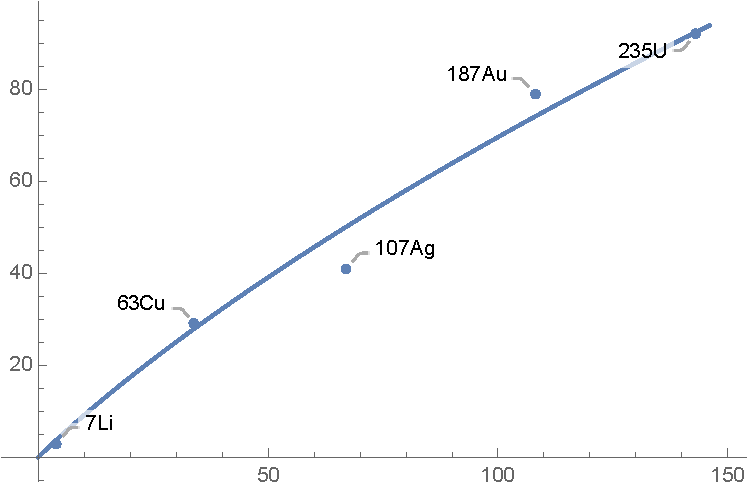
\includegraphics[width = 0.8\textwidth] {stabilitychart}

    \item \begin{enumerate}
        \item In all of these cases, there is an even number of neutrons, so they do not contribute to $j_{tot}$. For \ce{^39_{19} K _{20}}, there is a lone nucleon in the $1d_{3/2}$ state, so it has a total spin of $3/2$. For \ce{^{40}_{20}Ca_{20}}, the even number of protons means there is no net spin. For \ce{^{41}_{21} Sc_{20}}, there is again an unpaired nucleon in the $1d_{3/2}$ state, for a total spin of $3/2$.

        \item See attached page.

        \item \ce{^{12}C} has a $j_{tot}$ of $1/2$, since there is a single unpaired neutron in the $1p_{1/2}$ state, and no unpaired protons.

        \item \ce{^{13}N} has an even number of neutrons, so they do not contribute to $j_{tot}$. In the ground state, there is a single unpaired proton in the $1p_{1/2}$ state, for a total spin of $1/2$. When excited, this unpaired proton moves to the $1d_{5/2}$ level, for a total spin of $5/2$.
    \end{enumerate}

    \item \begin{enumerate}
        \item See attached page.

        \item Process ii. takes in heat, and process iv. expels it. Processes i and iii do not change the heat of the system.

        \item Let $P_1$ be the pressure at points $b$ and $c$, and let $P_2$ be the pressure at $a$ and $d$. If we are given the difference in pressure, $\Delta P$, and the distance between $a$ and $d$, the volume at $b$ and $c$ can be found. We have that
        \begin{equation*}
            P_1V_b^\gamma = P_2V_a^\gamma \implies V_b = V_a\left(\frac{P_2}{P_1}\right)^{1/\gamma}
        \end{equation*}
        \begin{equation*}
            P_1V_c^\gamma = P_2V_d^\gamma \implies V_c = V_d\left(\frac{P_2}{P_1}\right)^{1/\gamma}
        \end{equation*}
        Then the total work of the cycle is
        \begin{equation*}
            W = \oint P dV = \int_{V_a}^{V_b} P_2 \left(\frac{V_a}{V}\right)^\gamma dV + \int_{V_b}^{V_c} P_1 dV + \int_{V_c}^{V_d} P_1 \left(\frac{V_d}{V}\right)^\gamma dV + \int_{V_d}^{V_a} P_2 dV
        \end{equation*}
    \end{enumerate}


  \end{enumerate}


\end{document}
